\documentclass[12pt]{article}
%Gummi|065|=)
\usepackage{amsmath, amsfonts, amssymb}
\usepackage[margin=0.5in]{geometry}
\usepackage{xcolor}
%\usepackage{graphicx}
%\usepackage{graphicx}
\newcommand{\off}[1]{}
\DeclareMathSizes{20}{30}{21}{18}

\newcommand{\myhrule}{}

\newcommand{\dash}{
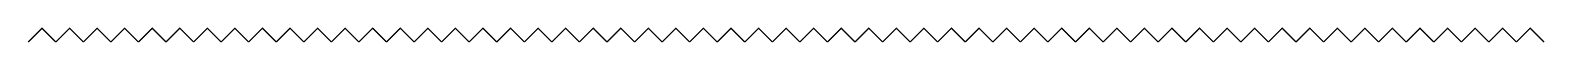
\begin{tikzpicture}[scale=0.35]
\foreach \x in {1,...,55}{
	\draw (\x,-0.25)--(\x+0.5,0.25)--(\x+1,-0.25);
}
\end{tikzpicture}
}

\usepackage{tikz}

\title{\textbf{ Examples:  $L^p$ spaces}}
\author{John D Mangual}
\date{}
\begin{document}

\fontfamily{qag}\selectfont \fontsize{25}{30}\selectfont

\maketitle

\noindent $L^2$ spaces are somewhat natural because we have Pythagoras theorem:
$$  \big|\big| (a,b)\big|\big|^2 = a^2 + b^2 $$
I have trouble understanding the meaning of the $L^p$ norms:
$$   \big( a^p + b^p \big)^{1/p}$$
I have no interpretation for them.  There's no picture I can draw.  \\ \\
There are a few starting points. Let $p,q \in (1, \infty)$ be related by
$$ \frac{1}{p} + \frac{1}{q}=1 $$
Then all measurable functions $f,g \geq 0$ satisfy:
$$ \int fg \, d\mu \leq \big|\big|f\big|\big|_p \, 
\big|\big|g\big|\big|_q $$
so for some reason this relationship of fractions gets promoted to a relationship of measurable functions. \\ \\
There is also Minkowski inequality:
$$ \big|\big| f + g \big|\big|_p \leq 
\big|\big| f  \big|\big|_p + 
\big|\big| g  \big|\big|_p $$
and it's downhill from there.  I have read in some places these have their origins in \textbf{convex gometry} in high dimensional space $\mathbb{R}^n$.  \\ \\
All the arguments I'm finding are pretty clumsy and not very geometric.  Instead we drown in a morass of
\begin{itemize}
\item poor disorganized writing
\item clumsy notation
\item non-visual thinking
\end{itemize}
I am concluding this subject is simply too difficult.  And going for my bike ride.

\newpage

\noindent Bourgain's Conjecture says for $a_\xi \in \mathbb{C}$ and $\epsilon > 0$ and $p \geq 6$:
$$
\big|\big| \sum_{\xi_1^2 +\xi_2^2 +\xi_3^2 =N^2 }
a_\xi e(\xi \cdot x) \big|\big|_{L^p(\mathbb{T}^n)}
\leq_\epsilon N^{\dots} \big|\big| a_\xi \big| \big|_{l^2\big(\{ \xi_1^2 + \xi_2^2 + \xi_3^2 = N^2 \}\big)}
 $$
 Some kind of Fourier series over points on the sphere is smaller than some average of the coefficients.  I could even write the left side:
 $$ \left[ \int_{[0,1]^3} \bigg|
 \sum_{\xi_1^2 +\xi_2^2 +\xi_3^2 =N^2 }
a_\xi e(\xi \cdot x) \bigg|^p \; dx
 \right]^{1/p}$$
 If I knew what these spaces where, I might have something intelligent to say here.  And I can't even type the correct inequality symbol it's not ``$\leq$". I don't know what Fourier restriction is.  And Bourgain's methods are just not visual or explicit enough. \\ \\
On the other hand if I'm this unhappy then I must certainly have something to way not in Bourgain-Demeter.

\newpage

\noindent 

\fontfamily{qag}\selectfont \fontsize{12}{10}\selectfont


\begin{thebibliography}{}

\item Jean Bourgain, Ciprian Demeter. \textbf{Proof of the $l^2$ Decoupling Conjecture} \texttt{ arXiv:1403.5335}


\end{thebibliography}



\end{document}